\documentclass{beamer}
\usetheme{Boadilla}
\usepackage{havannah}
\usepackage{color}
\newcommand{\hilight}[1]{\colorbox{yellow}{#1}}

\title[Learning MCTS]{Evolutionary Learning of Policies for MCTS Simulations}
\author[Pettit, Helmbold]{James Pettit, David Helmbold}
\institute[UCSC]{
  University of California, Santa Cruz\\
  \texttt{jpettit@soe.ucsc.edu}
}
\date[July 2012]{July 2012}

\begin{document}

\begin{frame}[plain]
  \titlepage
\end{frame}

\begin{frame}{Motivation}
\begin{enumerate}
	\item Cutting and connecting games are hard
	\item Computer Go - Next AI Grand Challenge
	\item Monte Carlo techniques promising
	\item Tuning policies difficult
	\item Solution: use evolution and self-play to learn better policies 
\end{enumerate}
\end{frame}

\begin{frame}{The Game of Hex - Good for AI}
	\begin{figure}[tb]
	\resizebox{3.3in}{!}{ \begin{HexBoard}[board size=7]
		  \HGame{}
		\end{HexBoard}
		}
	\end{figure}
	\begin{itemize}
		\item 2 player, perfect information
		\item Easy to program
		\item Clear-cut winning condition
		\item Large problem space
		\item Solved for boards up to 7x7
		\item Common sizes: 11x11, 13x13
	\end{itemize}
\end{frame}

\begin{frame}{The Game of Hex - Example Game}
	\begin{figure}[tb]
	\resizebox{3.3in}{!}{ \begin{HexBoard}[board size=7]
		  \HGame{d4}
		\end{HexBoard}
		}
	\end{figure}
	\begin{itemize}
		\item Connect opposing sides
		\item Cut opponents connections
	\end{itemize}
\end{frame}

\begin{frame}{The Game of Hex - Example Game}
	\begin{figure}[tb]
	\resizebox{3.3in}{!}{ \begin{HexBoard}[board size=7]
		  \HGame{d4,d3}
		\end{HexBoard}
		}
	\end{figure}
	\begin{itemize}
		\item Connect opposing sides
		\item Cut opponents connections
	\end{itemize}
\end{frame}

\begin{frame}{The Game of Hex - Example Game}
	\begin{figure}[tb]
	\resizebox{3.3in}{!}{ \begin{HexBoard}[board size=7]
		  \HGame{d4,d3,e3}
		\end{HexBoard}
		}
	\end{figure}
	\begin{itemize}
		\item Connect opposing sides
		\item Cut opponents connections
	\end{itemize}
\end{frame}

\begin{frame}{The Game of Hex - Example Game}
	\begin{figure}[tb]
	\resizebox{3.3in}{!}{ \begin{HexBoard}[board size=7]
		  \HGame{d4,d3,e3,f1}
		\end{HexBoard}
		}
	\end{figure}
	\begin{itemize}
		\item Connect opposing sides
		\item Cut opponents connections
	\end{itemize}
\end{frame}

\begin{frame}{The Game of Hex - Example Game}
	\begin{figure}[tb]
	\resizebox{3.3in}{!}{ \begin{HexBoard}[board size=7]
		  \HGame{d4,d3,e3,f1,c2}
		\end{HexBoard}
		}
	\end{figure}
	\begin{itemize}
		\item Connect opposing sides
		\item Cut opponents connections
	\end{itemize}
\end{frame}

\begin{frame}{The Game of Hex - Example Game}
	\begin{figure}[tb]
	\resizebox{3.3in}{!}{ \begin{HexBoard}[board size=7]
		  \HGame{d4,d3,e3,f1,c2,d6,b5,e2,c4,c3,a4,b6,c6,c5,d5,b7,c7,b4,a5,b3,a3,b1,b2,c1,d1}
		\end{HexBoard}
		}
	\end{figure}
	\begin{itemize}
		\item Connect opposing sides
		\item Cut opponents connections
	\end{itemize}
\end{frame}

\begin{frame}{Tree Search}
\begin{itemize}
	\item Game tree grows exponentially
	\begin{itemize}
		\item Hex on a general board is PSPACE-complete
	\end{itemize}
	\item No effective position evaluation heuristic
	\begin{itemize}
		\item \emph{Six}, previous champion until 2006, used circuit simulation
	\end{itemize}
	\item Limited opportunities for provable pruning
	\begin{itemize}
		\item \emph{MoHex}, current champion, does lots of this
	\end{itemize}
\end{itemize}
\end{frame}

\begin{frame}{Monte Carlo Tree Search}
\begin{itemize}
	\item Grow tree dynamically
	\item Use random playouts to estimate minimax value
	\item In the limit, converges to true minimax value
	\item Simple idea, remarkably successful
	\item Computationally expensive
\end{itemize}
\end{frame}

\begin{frame}{Monte Carlo Tree Search - Overview}
\begin{figure}
  \begin{center}
  \includegraphics[width=2.25in]{graphics/tree.pdf}
  \label{fig:encoding}
  \end{center}
\end{figure}
\begin{itemize}
	\item \emph{Select} - using win/loss statistics, traverse tree to a leaf
	\item {\bf Playout} - from selected position, \emph{randomly} play out game until final position
	\item \emph{Update} - using results of playout, update win/loss statistics
\end{itemize}
\end{frame}

\begin{frame}{Monte Carlo Tree Search - Playout Policies}
\begin{itemize}
	\item Playout policy a critical part of overall performance
	\item We examine 4 different policies:
	\begin{itemize}
		\item Default - uniform random
		\item Uniform Local - play in local neighborhood first
		\item Uniform Local with Tenuki (Play-Away) - possibly play in local neighborhood first
		\item Local Pattern Weighted - stochastic, weighted local neighborhood
	\end{itemize}
\end{itemize}
\end{frame}

\begin{frame}{Weighting the Playout Policy}
\begin{figure}
  \begin{center}
  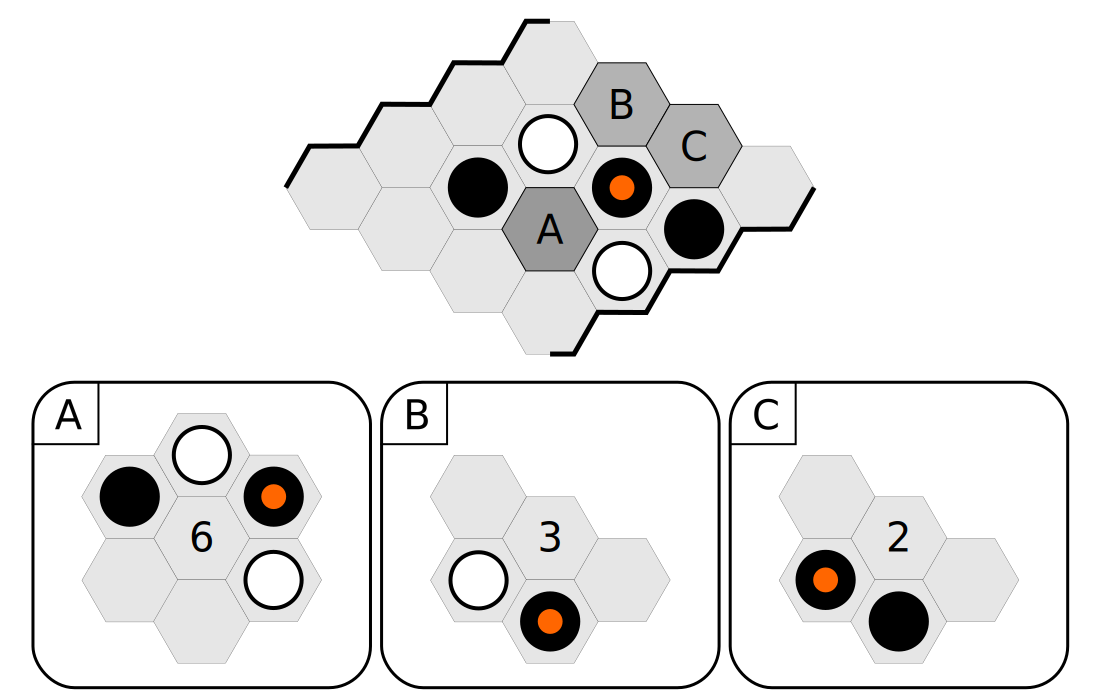
\includegraphics[width=3.25in]{graphics/local-pattern.pdf}
  \label{fig:encoding}
  \end{center}
\end{figure}
\begin{itemize}
	\item Use patterns to weight moves
	\item Weight moves local to last-played move
	\item If local area is filled, use default policy
\end{itemize}
\end{frame}

\begin{frame}{Example Encoding}
\begin{figure}
  \begin{center}
  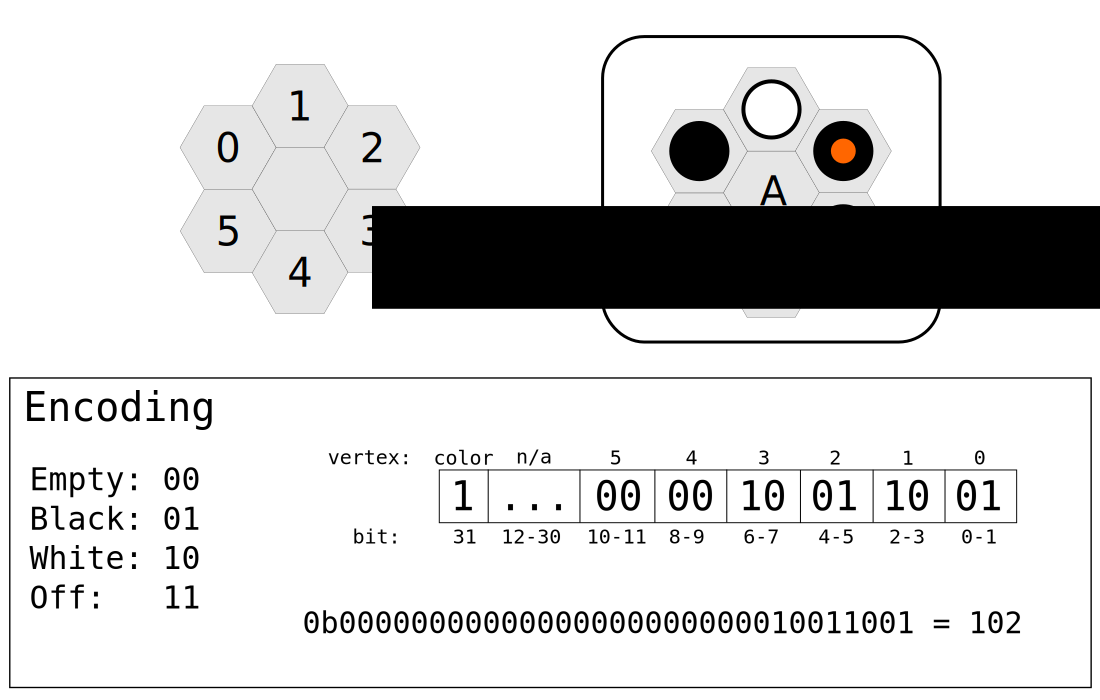
\includegraphics[width=3.25in]{graphics/weight-pattern-map.pdf}
  \label{fig:encoding}
  \end{center}
\end{figure}
\begin{itemize}
	\item Fast lookup table mapping pattern to weight
	\item Plenty of unused space in upper bits for storing extra info
\end{itemize}
\end{frame}

\begin{frame}{Monte Carlo Tree Search - Playout Policy}
\begin{itemize}
	\item Execution time is critical
	\item Requires deep insight to develop weights, then careful and expensive testing to verify improvement
	\item Naively ``improving'' the strength of the playout policy can hurt overall performance
	\begin{itemize}
		\item Subtle interaction between selection, update, and playout
		\item Example: fully deterministic policy equivalent to an evaluation function
	\end{itemize}
	\item We want a technique to learn weights automatically
\end{itemize}
\end{frame}

\begin{frame}{Evolutionary Learning}
\begin{itemize}
	\item Idea: Evolve playout policy
	\item Policy = set of all possible local patterns + weights for those patterns
	\item Individual policies compete via self-play to propagate
	\item Best individuals are selected for reproduction
	\item Mutation/recombination operates on individual's pattern weights
	\item Individuals play \emph{complete} games against each other using \emph{complete} MCTS system
\end{itemize}
\end{frame}

\begin{frame}{Evolution}
\begin{itemize}
	\item Init
	\begin{enumerate}
		\item Generate $n$ individuals (population)
	\end{enumerate}
	\item Each Generation
	\begin{enumerate}
		\item Evaluate fitness
		\item Rank by fitness
		\item Select top $c$ individuals, $c < n$
		\item Recombine individuals into $n$ new children
		\item Mutate children
	\end{enumerate}
\end{itemize}
\end{frame}

\begin{frame}{Results of learning after training on 7x7}
\begin{figure}
	\caption{Trained on 7x7 board}
	\begin{center}
		\begin{tabular}{c | c c c}
		& \multispan{3}{\hfil opponent \hfil} \\
		 player & default & uniform local & uniform local (tenuki) \\
		\hline
		uniform local & 70.50\% & & \\
		uniform local (tenuki) & 61.00\% & 50.00\% & \\
		learned & \hilight{90.00\%} & \hilight{84.00\%} & \hilight{86.00\%} \\
		\end{tabular}
	\label{fig:results}
	\end{center}
\end{figure}
\begin{itemize}
	\item All-play-all tournament of the 4 policy variants.
	\item Each element is the percent win-rate of the row variant versus the column variant.
	\item 200 games per pair.
\end{itemize}
\end{frame}

\begin{frame}{Generalization to Different Board Sizes}
\centerline{
\begin{tabular}{c | cc cc}
 & \multispan{2}{\hfil default \hfil} & \multispan{2}{\hfil uniform local\hfil} \\
 & 11x11 & 13x13 & 11x11 & 13x13 \\ \hline
 learned & 92.5 \% & 94 \%  & 88.5\% & 85\%
 \end{tabular}
}
\begin{figure}
\caption{Trained on 7x7 board}
	\begin{center}
		\begin{tabular}{c | c c}
		& default & uniform local \\
		\hline
		learned & 90.00\% & 84.00\% \\
		\end{tabular}
	\label{fig:results}
	\end{center}
\end{figure}
\end{frame}

\begin{frame}{Results versus MoHex}
\begin{figure}
	\begin{center}
		\begin{tabular}{c | c}
		& MoHex on 7x7 \\
		\hline
		default & 11.75\% \\
		uniform local & 26\% \\
		learned & 42\% \\
		\end{tabular}
	\end{center}
\end{figure}
\begin{figure}
	\begin{center}
		\begin{tabular}{c  | c c c}
		& MoHex on 11x11 & Relative CPU \\
		\hline
		default & 0.5\% & 100\% \\
		uniform local & 0.0\% & 107\% \\
		learned & 11\% & 122\% \\
		\end{tabular}
	\end{center}
\end{figure}
\begin{itemize}
	\item MoHex, the current world-champion, uses lots of expert and domain-specific knowledge
	\item Good results on small board
	\item Dramatic improvement for modest overhead
\end{itemize}
\end{frame}

\begin{frame}{Conclusion}
\begin{itemize}
	\item Computer Hex/Go present a huge problem space
	\item MCTS is an effective technique to navigate that space
	\item Shown we can automatically learn to guide MCTS to play computer Hex better
	\item Future work - apply results to different games
	\item Source code available at \url{https://github.com/etherealmachine/hivemind}
\end{itemize}
\end{frame}

\begin{frame}{Conclusion}
\centerline{Thank you for the time}
\centerline{Questions?}
\end{frame}

\end{document}
